\documentclass{article}
\usepackage[utf8]{inputenc}
\usepackage{geometry} 
\geometry{letterpaper}
\usepackage{graphicx}	
\usepackage{amssymb}\setlength{\parindent}{0pt}
\title{HW7-Notes}
\date{March 2020}
\author{Yiping Lu and Jody Shu}

%\date{}							% Activate to display a given date or no date

\begin{document}
\begin{Large}
\maketitle
\section{Softmax Regression Algorithm}
%\subsection{}

Softmax is an extension of Logistic Regression (LR).

LR setup : $y \in \{0,1\} \leftarrow discrete$\\
want: $h_\theta \in [0,1]$
\begin{figure}[h] %  figure placement: here, top, bottom, or page
   \centering
   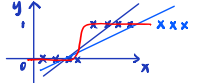
\includegraphics[width=3in]{logisticRegressionPlot} 
\end{figure}
\\
Linear reg: [ -$\infty, \infty$ ]\\
Choose:  $h_\theta (x)=g(\theta^T x)= \frac{1}{1+e^{-\theta^Tx}}$ ,
\\
where $g(z)=\frac{1}{1+e^{-z}}$
\\ (note: $z\rightarrow -\infty \ g(z), \rightarrow 0$,\\
            $\hspace{30pt} z\rightarrow \infty \ g(z), \rightarrow 1)$\\
g is called sigmoid/Logistic function\\
Here: g:$(-\infty, \infty) \rightarrow (0,1)$

p(y=1$\mid x; \theta)=h_\theta (x)=\frac{1}{1+e^{-\theta ^T x}}$\\
p(y=0$\mid y; \theta)=1-h_\theta (x) \geq 0 \ (0 \leq h_\theta (x) \leq 1)$
\\
Next, we are going to write the prob. fcn into one equation.

$p(y\mid x; \theta)=h_\theta(x)^y(1-h_\theta(x))^{1-y}\\
y=1\Rightarrow p(y=1\mid x; \theta)=h_\theta(x)^1(1-h_\theta(x))^{0}\\
y=0\Rightarrow p(y=0\mid x; \theta)=1-h_\theta(x)\\
L(\theta)=p(y=0\mid x; \theta)=\prod_{i} p(y^{i}\mid x^{i}; \theta)=\prod_{i} h_\theta(x^{i})^{y^{i}}(1-h_\theta(x^{i}))^{1-y^{i}})$\\
It is much easier to maximize the log likelihood.\\
$l(\theta)=log L(\theta)=\sum_{i} [y^{i}log h_\theta(x^{i})+(1-y^{i})log (1-h_\theta(x^{i}))]\\$
How to maximize it? Use (stochastic) gradient descent.\\
$\theta:=\theta\bigoplus\alpha\nabla_\theta l(\theta)$\\
$\bigoplus$: along with the gradient direction.\\
$\frac{\partial }{\partial \theta_j} l(\theta) = \sum_{i=1}^{n} (y^{i}-h_\theta(x^{i}))x_j^{i} $

\end{Large}
\end{document}